\documentclass[10pt]{beamer}
\usetheme[progressbar=frametitle]{metropolis}
\usepackage{appendixnumberbeamer}
\usepackage[spanish]{babel}
\usepackage[utf8]{inputenc}
\usepackage{booktabs}
\usepackage{graphicx}
\usepackage[scale=2]{ccicons}
\usepackage{hyperref}
\usepackage{multimedia}
\usepackage{graphicx}
\usepackage{pgfplots}
\usepgfplotslibrary{dateplot}
\usepackage{xspace}
\usepackage[
    type={CC},
    modifier={by-sa},
    version={4.0},
]{doclicense}
\newcommand{\themename}{\textbf{\textsc{metropolis}}\xspace}
\title{Beamer}
\subtitle{Presentaciones con \LaTeX}
\date{\today}
\author{Gustavo Castro}
% \institute{Institución}

\begin{document}
\maketitle

\begin{frame}{Contenido}
    \setbeamertemplate{section in toc}[sections numbered]
    \tableofcontents[hideallsubsections]
\end{frame}

\section{Introducción}

\begin{frame}[fragile]{¿Qué es Beamer?}

\textbf{Beamer} es una clase para \LaTeX que permite crear presentaciones flexibles y vistosas, incluyendo todas las secciones que se esperan en ese tipo de documentos: títulos en cada diapositiva, resaltado de ciertos elementos, tablas de contenidos y efectos entre páginas, además de todas potencia que ofrece \LaTeX. Este mismo documento se creó con ese paquete.
\\ \vspace{0.3in}
Código fuente: \\
\url{https://github.com/josephwright/beamer}
\\ \vspace{0.3in}Aprender sobre el uso de Beamer: \url{https://www.sharelatex.com/learn/Beamer}
\end{frame}

\begin{frame}[fragile]{Temas}
\begin{verbatim}
    \documentclass{beamer}
    \usetheme{metropolis}
\end{verbatim}
\end{frame}
\begin{frame}[fragile]{Secciones}
Al especificar secciones, cada diapositiva se agrupa dentro del tema correspondiente

\begin{verbatim}
    \section{Sección de ejemplo}
\end{verbatim}

El tema usado en esta presentación, \themename, muestra una barra de progreso:
\end{frame}

\section{Títulos}
\begin{frame}{Metropolis titleformats}
Este tema en particular soporta cuatro formatos de título distintos:
    \begin{itemize}
        \item Regular
        \item \textsc{Smallcaps}
        \item \textsc{allsmallcaps}
        \item ALLCAPS
    \end{itemize}
Esto puede establecerse para todo el documento individualmente para títulos en específico.
\end{frame}

\section{Elementos}

\begin{frame}[fragile]{Formateo del texto}
\begin{verbatim}
También se puede formatear el texto para resaltar ciertos
elementos. Por ejemplo, \emph{enfatizar} ciertas palabras,
hacer notar \alert{alertas}o mostrar el texto en
\textbf{negritas}.
\end{verbatim}

\begin{center}que se resulta en\end{center}
También se puede formatear el texto para resaltar ciertos elementos. Por ejemplo, \emph{enfatizar} ciertas palabras, hacer notar \alert{alertas} o mostrar el texto en \textbf{negritas}.
\end{frame}

\begin{frame}{Estilo del texto}
  \begin{itemize}
    \item Regular
    \item \textit{Cursivas}
    \item \textsc{SmallCaps}
    \item \textbf{Negritas}
    \item \textbf{\textit{Negritas en crusiva}}
    \item \textbf{\textsc{SmallCaps en negritas}}
    \item \texttt{Ancho fijo}
    \item \texttt{\textit{Ancho fijo en cursivas}}
    \item \texttt{\textbf{Ancho fijo en negritas}}
    \item \texttt{\textbf{\textit{Ancho fijo en negritas y cursivas}}}
  \end{itemize}
\end{frame}

\begin{frame}{Listas}
  \begin{columns}[T,onlytextwidth]
    \column{0.33\textwidth}
      Ingredientes
      \begin{itemize}
        \item Leche \item Huevos \item Harina
      \end{itemize}

    \column{0.33\textwidth}
      Numeraciones
      \begin{enumerate}
        \item Primero, \item Segundo y \item Tercero.
      \end{enumerate}

    \column{0.33\textwidth}
      Descripciones
      \begin{description}
        \item[PowerPoint]: 
\includegraphics[scale=.1]{down} \item[Beamer]: 
\includegraphics[scale=.1]{up}
      \end{description}
  \end{columns}
\end{frame}
\begin{frame}{Animaciones}
  \begin{itemize}[<+- | alert@+>]
    \item \alert<4>{Estos es\only<4>{ muy} importante}
    \item También esto
    \item Y esto otro
  \end{itemize}
\end{frame}
\begin{frame}{Figuras}
  \begin{figure}
    \newcounter{density}
    \setcounter{density}{20}
    \begin{tikzpicture}
      \def\couleur{alerted text.fg}
      \path[coordinate] (0,0)  coordinate(A)
                  ++( 90:5cm) coordinate(B)
                  ++(0:5cm) coordinate(C)
                  ++(-90:5cm) coordinate(D);
      \draw[fill=\couleur!\thedensity] (A) -- (B) -- (C) --(D) -- cycle;
      \foreach \x in {1,...,40}{%
          \pgfmathsetcounter{density}{\thedensity+20}
          \setcounter{density}{\thedensity}
          \path[coordinate] coordinate(X) at (A){};
          \path[coordinate] (A) -- (B) coordinate[pos=.10](A)
                              -- (C) coordinate[pos=.10](B)
                              -- (D) coordinate[pos=.10](C)
                              -- (X) coordinate[pos=.10](D);
          \draw[fill=\couleur!\thedensity] (A)--(B)--(C)-- (D) -- cycle;
      }
    \end{tikzpicture}
    \caption{Esta imagen fue rotada usando \LaTeX. Original en  
    \href{http://www.texample.net/tikz/examples/rotated-polygons/}{texample.net}.}
  \end{figure}
\end{frame}
\begin{frame}{Tablas}
  \begin{table}
    \caption{Ciudades más grande en el mundo (fuente: Wikipedia)}
    \begin{tabular}{cr cr lr}
      \toprule
      Ciudad & País & Población\\
      \midrule
      Tokyo–Yokohama & Japón & 37,750,000\\
      Jakarta & Indonesia & 30,091,131\\
      Seoul & Corea del Sur & 15,796,450\\
      Delhi & India & 24,998,000\\
      \bottomrule
    \end{tabular}
  \end{table}
\end{frame}
\begin{frame}{Bloques}

  \begin{columns}[T,onlytextwidth]
    \column{0.5\textwidth}
      \begin{block}{Defecto}
        Contenido.
      \end{block}

      \begin{alertblock}{Alerta}
        Contenido.
      \end{alertblock}

      \begin{exampleblock}{Otro}
        Contenido.
      \end{exampleblock}

    \column{0.5\textwidth}

      \metroset{block=fill}

      \begin{block}{Defecto}
        Contenido.
      \end{block}

      \begin{alertblock}{Alerta}
        Contenido.
      \end{alertblock}

      \begin{exampleblock}{Otro}
        Contenido.
      \end{exampleblock}

  \end{columns}
\end{frame}
\begin{frame}{Matemáticas}
  \begin{equation*}
    e = \lim_{n\to \infty} \left(1 + \frac{1}{n}\right)^n
  \end{equation*}
\end{frame}
\begin{frame}{Gráficas}
  \begin{figure}
    \begin{tikzpicture}
      \begin{axis}[
        mlineplot,
        width=0.9\textwidth,
        height=6cm,
      ]

        \addplot {sin(deg(x))};
        \addplot+[samples=100] {sin(deg(2*x))};

      \end{axis}
    \end{tikzpicture}
  \end{figure}
\end{frame}
\begin{frame}{Gráficas de barras}
  \begin{figure}
    \begin{tikzpicture}
      \begin{axis}[
        mbarplot,
        xlabel={Foo},
        ylabel={Bar},
        width=0.9\textwidth,
        height=6cm,
      ]

      \addplot plot coordinates {(1, 20) (2, 25) (3, 22.4) (4, 12.4)};
      \addplot plot coordinates {(1, 18) (2, 24) (3, 23.5) (4, 13.2)};
      \addplot plot coordinates {(1, 10) (2, 19) (3, 25) (4, 15.2)};

      \legend{lorem, ipsum, dolor}

      \end{axis}
    \end{tikzpicture}
  \end{figure}
\end{frame}
\begin{frame}{Citas}
  \begin{quote}
    Lorem ipsum dolor sit amet, consectetur adipiscing elit, sed do eiusmod tempor incididunt ut labore et dolore magna aliqua.
  \end{quote}
\end{frame}

{%
\setbeamertemplate{frame footer}{Pie de página personalizado}
\begin{frame}[fragile]{Referencias al pie de la diapositiva}
    \themename incluye una plantilla personalizada para agregar texto al pie de las páginas. Se agrega con:
    \begin{verbatim}\setbeamertemplate{frame footer}{Pie de página personalizado}\end{verbatim}
\end{frame}
}

\section{Multimedia}
\begin{frame}{Videos}
\begin{figure}[h!]
\centering
\movie[label=show3,width=0.5\textwidth,poster
       ,autostart,showcontrols,loop] 
  {
\includegraphics[width=0.5\textwidth]{video.png}}{video.mp4}
  \caption{Video de prueba insertado con el paquete \texttt{multimedia}}
 \end{figure}
\end{frame}

\begin{frame}{Audio}
\begin{figure}[h!]
\centering    
\movie[label=show3,width=0.5\textwidth,poster
       ,autostart,showcontrols,loop] 
  {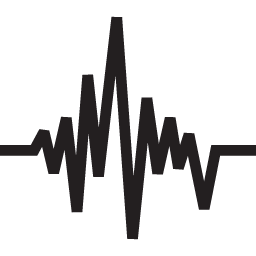
\includegraphics[width=0.5\textwidth]{audio.png}}{audio.m4a}
  \caption{Audio de prueba insertado con el paquete \texttt{multimedia}}
 \end{figure}
\end{frame}

\section{¿Por qué usar Beamer?}
\begin{frame}{Ventajas}
    \begin{itemize}
        \item Mayor y mejor control
        \item Independencia de plataforma
        \item Documentos universales
        \item Matemáticas
        \item Auto-contención
        \item Estandarizado
        \item Completamente libre y gratuito
    \end{itemize}
\end{frame}

\begin{frame}{Desventajas}
    \begin{itemize}
        \item Mayor curva de aprendizaje
        \item No es WYSIWYG
        \item Uso no muy difundido
    \end{itemize}
\end{frame}

\section{Conclusiones}
\begin{frame}{Distribución}
    \doclicenseThis
    Fuente: \url{https://gustawho.com/beamer.zip}
\end{frame}

\end{document}
